\documentclass{beamer}

%style
\mode<presentation>{
	%\usetheme{Goettingen}
	\usetheme{default}
}
%packages
\usepackage[utf8]{inputenc}
\usepackage[ngerman]{babel}
\usepackage{graphicx}

%
% packages.tex -- zusätzliche Packages 
%
% In diesem File werden \usepackage{}-Aufrufe eingetragen für Packages, die
% noch nicht im skript.tex aufgerufen werden
%
% (c) 2018 Michael Müller, Hochschule Rapperswil
%



%Einstellungen Präsentation
\title{Klima auf anderen Planeten}
\author{Nicolas Tobler}
\institute{Mathematisches Seminar 2018}
\date{14.05.2018}

%Bilder
\graphicspath{{Pictures/}}

%Beginn der Präsentation
\begin{document}

%Titelseite
\begin{frame}
\titlepage
\end{frame}

%Inhaltsverzeichnis
\begin{frame}
\frametitle{Inhalt}
\tableofcontents
\end{frame}

\section{Einführung}

\subsection{Planeten im Vergleich}
\begin{frame}
	\frametitle{Planeten im Vergleich}
	
	\begin{figure}
	\center
	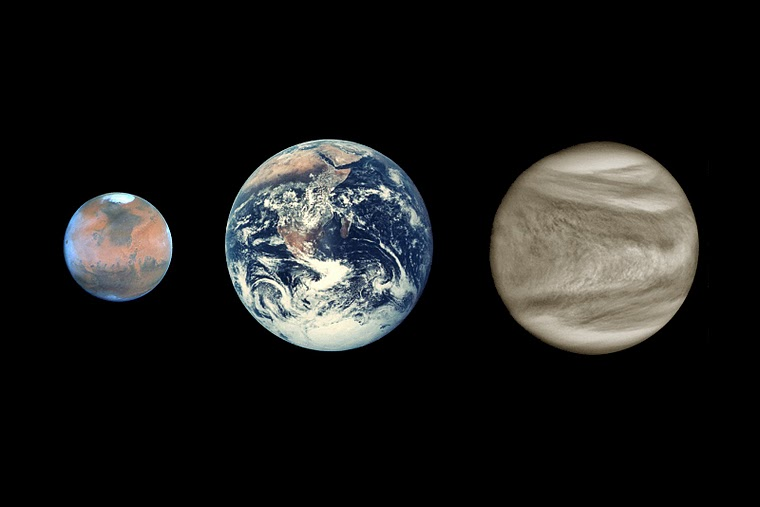
\includegraphics[width=0.7\linewidth]{planets.jpg}
	\end{figure}
	
\begin{columns}
\begin{column}{0.33\textwidth}
   Mars
   \begin{itemize}
   		\item[-] Kaum Wolken
   		\item[-] Heiss
   \end{itemize}
\end{column}
\begin{column}{0.33\textwidth}
   Venus
   \begin{itemize}
   		\item[-] Dicke Wolkendecke
   		\item[-] Heiss
   \end{itemize}
\end{column}
\begin{column}{0.33\textwidth}
   Erde
   \begin{itemize}
   		\item[-] Normales Wetter
   \end{itemize}
\end{column}
\end{columns}

\end{frame}

\subsection{Ziel}
\begin{frame}
\frametitle{Ziel}
\begin{itemize}
	\item[] Werdegang der Planeten nachvollziehen
	\item[] Annahmen
	\begin{itemize}
	\item[-] Gleiche Vorausbedingugnen
	\end{itemize}
\end{itemize}
\end{frame}


\section{Modell} 
\begin{frame}
	\frametitle{Modell}
	\begin{figure}
		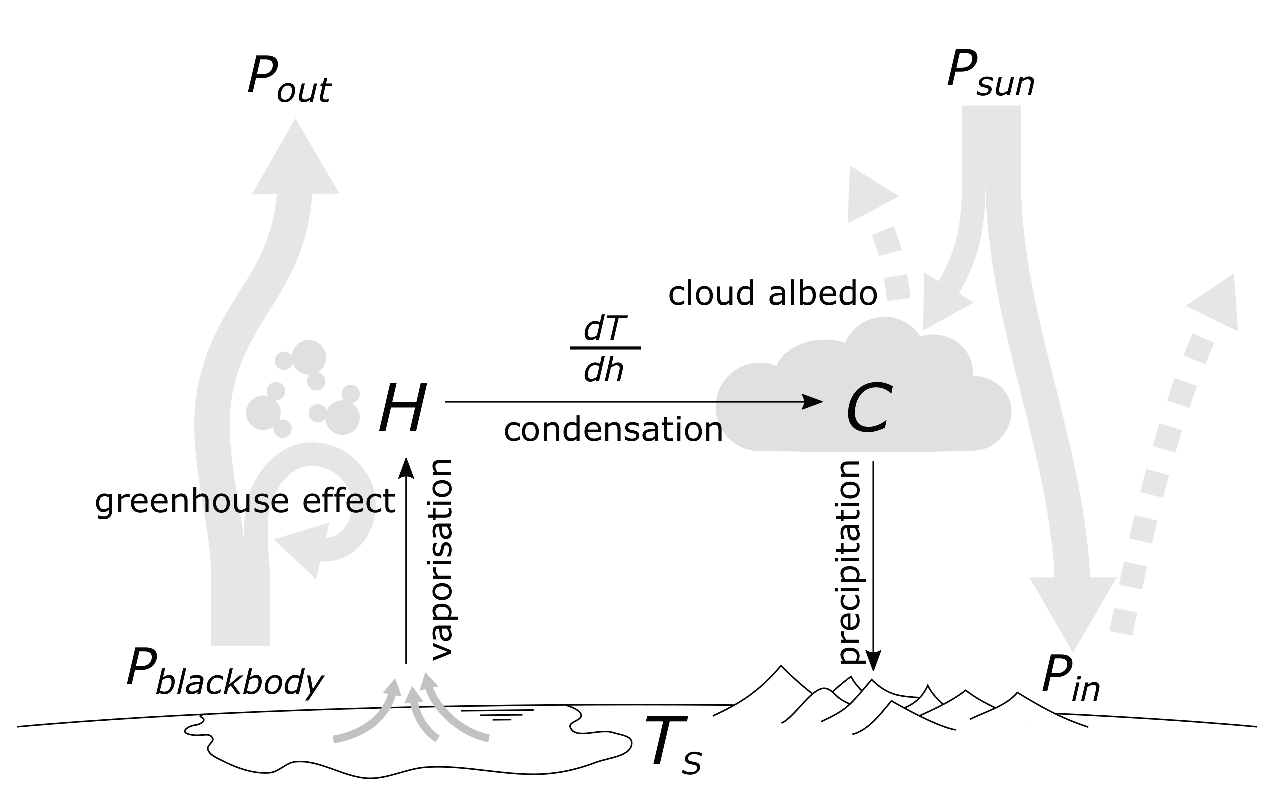
\includegraphics[width=\linewidth]{Model.eps}
	\end{figure}
\end{frame}

\subsection{Energiehaushalt}
\begin{frame}
\frametitle{Energiehaushalt}
\begin{itemize}
	\item[] Absorbierte Leistung
	\begin{equation}
	P_{in} = \sigma T_{\astrosun}^4 \left( \frac{R_{\astrosun}}{a_{planet}} \right) ^2 \cdot (1-\alpha)
	\end{equation}
	\pause
	
	\item[] Abgestrahlte Leistung
	\begin{equation}
	P_{out} = (4 \pi R_{S}^2 \sigma T_{S}^4)(1 - \beta)
	\end{equation}
	\pause
	
	\item[] Albedo
	\begin{equation}
	\alpha(C) = (0.65 \cdot C) + 0.15;
	\end{equation}
	\pause
	
	\item[] Treibhauseffekt
	\begin{equation}
	\beta(H) = 0.5 \cdot H
	\end{equation}
\end{itemize}
\end{frame}




\subsection{Wasserkreislauf}

\begin{frame}
	\frametitle{Wasserkreislauf}
	\begin{itemize}
		\item[] Wasserdampfbildung
			\begin{equation}
			p_5 (P_{in})
			\end{equation} 
		\pause
		\item[] Wolkenbildung
			\begin{equation}
			p_6 \left( H \frac{dT}{dh} \right)
			\end{equation}
		\pause
		\item[] Wolkenabbau 
		 	\begin{equation}
			p_5 (C)
			\end{equation}
	\end{itemize}
\end{frame}

\begin{frame}
	\frametitle{Wasserkreislauf}
	\begin{itemize}
	
		\item[] Wasserkreislauf
			\begin{equation}
			\dot{H} = p_5 (P_{in}) - p_4 \left( H \frac{dT}{dh}) \right)
			\end{equation}
			\begin{equation}	
			\dot{C} = p_4 \left( H \frac{dT}{dh} \right) - p_5 C
			\end{equation}		
	
		\item[] Temperaturgradent
			\begin{equation}
			\frac{dT}{dh} \approx \xi (T_S - T_T)
			\end{equation}
		
		\item[] Eingesetzt
			\begin{equation}
			\dot{H} = p_5 (P_{in}) - p_4 \left( H(T_S - T_T) \right)
			\end{equation}
			\begin{equation}	
			\dot{C} = p_4 \left( H(T_S - T_T) \right) - p_5 C
			\end{equation}		
		
	\end{itemize}
\end{frame}

\subsection{Temperaturgradient}

\begin{frame}
	\frametitle{Temperaturgradient}
	\begin{itemize}
		\item[] Oberflächentemperatur
		
			\begin{equation}
			\dot{T_S} = p_1 \left( P_{in}(C) - P_{out}(T_S, H) \right)
			\end{equation}
		\item[] Tropopausentemperatur
			\begin{equation}	
			\dot{T_T} = p_2 \left( P_{in}(C) \cdot H \right) - P_{blackbody}(T_T) - p_3 \left( (T_T - T_S) \cdot H \right)
			\end{equation}		
		
	\end{itemize}
\end{frame}

\subsection{Zusammengefasste Gleichungen}

\begin{frame}
\frametitle{Zusammengefasste Gleichungen}
\begin{itemize}
	\item[] Zusammengefasst
	
\begin{equation}
\left|
\begin{array}{lcl}
\dot{T}_S = p_1 \left( P_{in}(C) - P_{out}(T_S, H) \right) \\
\dot{T}_T = p_2 \left( P_{in}(C) \cdot H \right) - P_{blackbody}(T_T) - p_3 \left( (T_T - T_S) \cdot H \right) \\
\dot{C} = p_4 \left( H(T_S - T_T) \right) - p_5 C \\
\dot{H} = p_5 \left(P_{in} \right) - p_4 \left( H(T_S - T_T) \right)
\end{array}
\right|
\end{equation}
	
	\pause
	
	\item[] Mit limitierenden Termen
	
\begin{equation}
\left|
\begin{array}{lcl}
\dot{T}_S = p_1 \left( P_{in}(C) - P_{out}(T_S, H) \right) \\
\dot{T}_T = p_2 \left( P_{in}(C) \cdot H \right) - P_{blackbody}(T_T) - p_3 \left( (T_T - T_S) \cdot H \right) \\
\dot{C} = p_4 \left( (H + H^9)(T_S - T_T) \right) - p_5 (C + C^5) \\
\dot{H} = p_5 \left(P_{in} \right) - p_4 \left( (H + H^9 )(T_S - T_T) \right)
\end{array}
\right|
\end{equation}

\end{itemize}
\end{frame}

\section{Simulationsergebnisse}

\subsection{Temperatur}
\begin{frame}
	\frametitle{Temperatur}
		\begin{figure}
			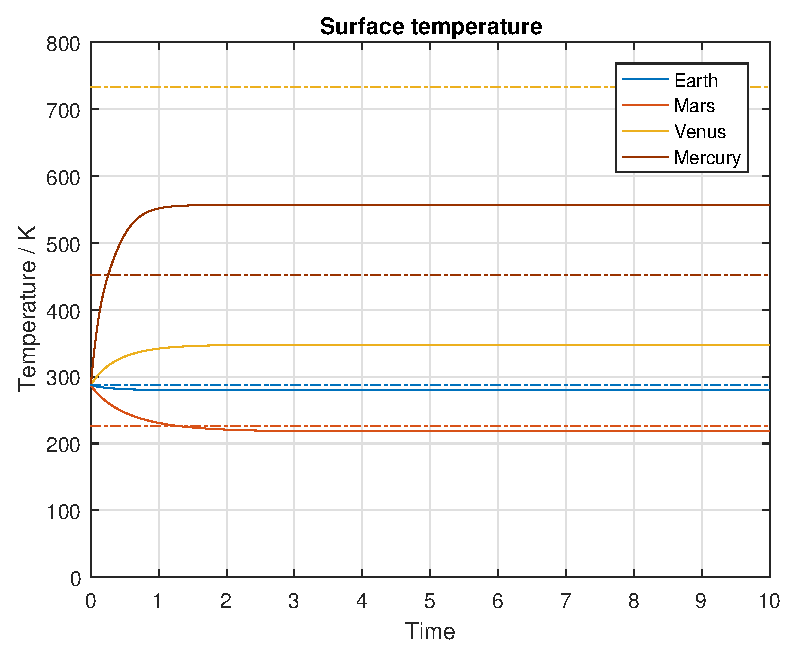
\includegraphics[width=\linewidth]{Matlab/figures/surfaceTemperature.eps}
		\end{figure}
\end{frame}

\subsection{Luftfeuchtigkeit}
\begin{frame}
	\frametitle{Luftfeuchtigkeit}
		\begin{figure}
			\includegraphics[width=\linewidth]{Matlab/figures/humidity.eps}
		\end{figure}
\end{frame}

\subsection{Wolkenabdeckung}
\begin{frame}
	\frametitle{Wolkenabdeckung}
		\begin{figure}
			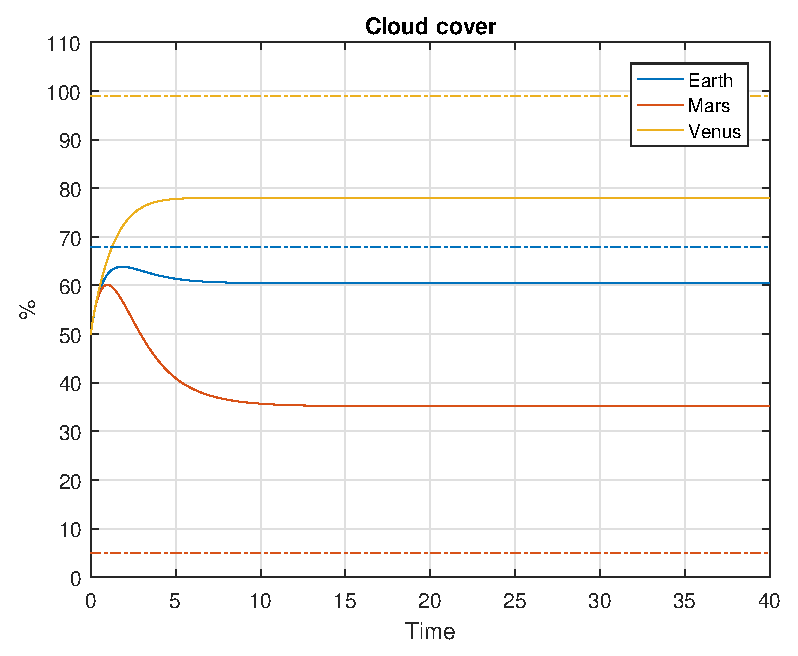
\includegraphics[width=\linewidth]{Matlab/figures/cloudCover.eps}
		\end{figure}
\end{frame}

\subsection{Albedo}
\begin{frame}
	\frametitle{Albedo}
		\begin{figure}
			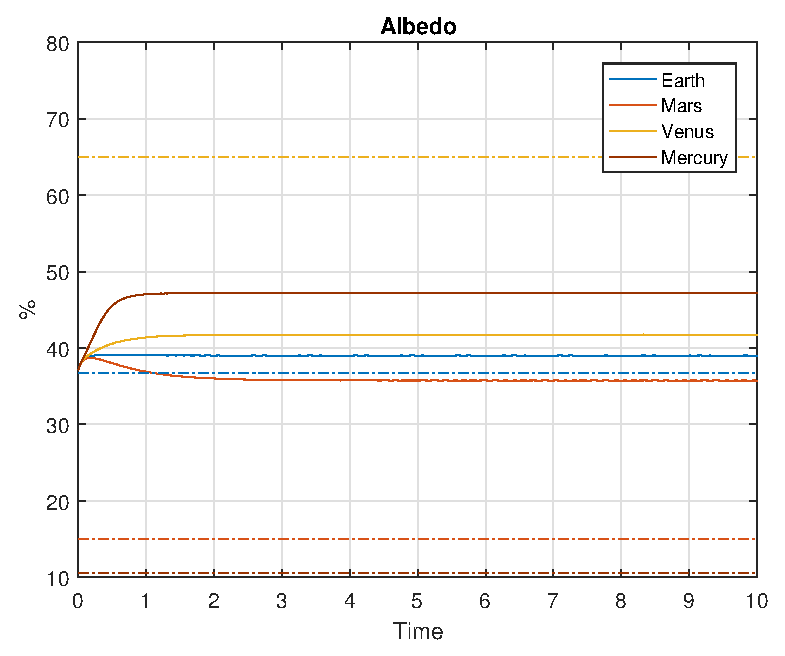
\includegraphics[width=\linewidth]{Matlab/figures/albedo.eps}
		\end{figure}
\end{frame}

\subsection{Fazit}
\begin{frame}
\frametitle{Fazit}
\begin{itemize}
	\item[] Gleichung mit Dämpfung
	\begin{equation}
	\dot{T}(t)=-cT(t)+aT(t-\frac{1}{2}\tau_K)-bT(t-(\frac{1}{2}\tau_R+\tau_K))-\epsilon(T(t))^3
	\end{equation}
	\pause
	\item[] Änderung des Parameters a
	
\end{itemize}
\end{frame}

\end{document}